\section{Sparse DETR: Efficient End-to-End Object Detection with Learnable Sparsity}

\label{appendix:sparse-detr-paper}

\subsection{Overview}

\par Roh \textit{et al} in their 2021 paper \textit{Sparse DETR: Efficient End-to-End Object Detection with Learnable Sparsity} aims to solve the bottleneck of Deformable DETR by sparsifying the encoder token by using DAM (Decoder Attention Map) predictor \cite{roh2021sparse}.

\subsection{Methodology}
\subsubsection{Encoder Token Sparsification} 
\par In token sparsification scheme, the encoder module selectively refines a small number of encoder tokens. This encoder token subset is obtained from the backbone feature map $X_{feat}$ with a certain criterion like Decoder Cross-Attention Map (DAM). For features that are not updated in this process, the values of $X_{feat}$ are passed through the encoder layers without being changed

\begin{figure}[h]
	\centering
	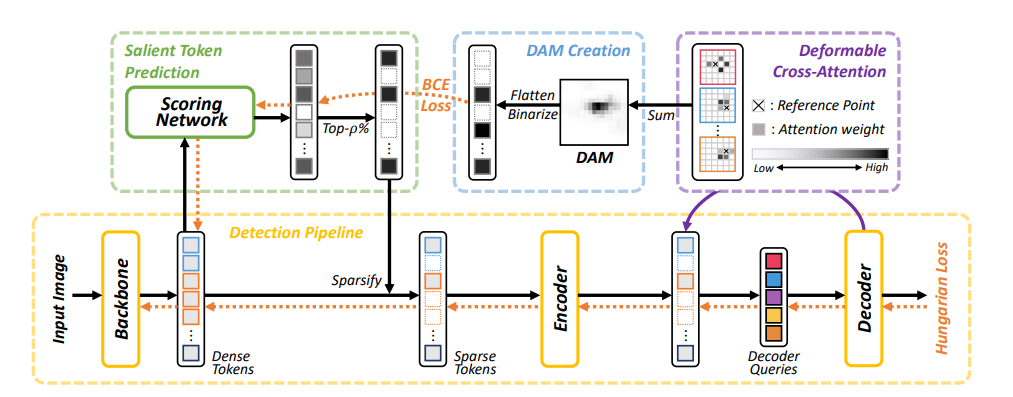
\includegraphics[width=\linewidth]{assets/img/sparse-detr-dam.png}
	\caption{ Decoder Cross Attention Map (DAM) by Rho
		\textit{et al} (Courtesy \cite{roh2021sparse})}
\end{figure}

\subsubsection{Decoder Cross-Attention Map}
\begin{itemize}
	\item A cross attention map from the transformer decoder is used to find the salient tokens.
	\item A scoring network is used to determine which encoder tokens should be further modified on the fly by predicting a pseudo ground truth of the saliency defined by decoder cross-attention maps.
	\item The saliency of each input token is determined by aggregating the decoder cross-attentions between all object queries and the encoder output. It generates a single map of the same size as the backbone's feature map, which is known as the Decoder cross Attention Map (DAM).
	\item To train the scoring network, we binarize DAM so that only the top-k percentage of encoder tokens are kept. This is because the goal is to find a small subset of encoder tokens that the decoder references the most, rather than predicting how many times each encoder token will be referenced by the decoder.
	\item To predict how likely a given encoder token is to be included in the top-p \% most referenced tokens, a 4-layer scoring network g is used, and the network is trained by minimizing the binary cross entropy (BCE) loss between the binarized DAM and prediction.
	
	$$ L_{dam} = -\frac{1}{N}\displaystyle\sum\limits_{i=1}^N BCE(g(X_{feat})_i, DAM^{bin}_i) 
	$$
\end{itemize}

\subsubsection{Encoder Auxiliary Loss}
\par Auxiliary loss can be applied to the encoder layers without sacrificing too much computational effort because the sparse detr model has a sparsified token set. Apart from better efficiency and performance, the encoder auxiliary loss has another advantage: it allows to stack more encoder layers safely without failing to converge.


\subsection{Conclusion}
\par Roh \textit{et al} propose the encoder token sparsification method, which reduces the encoder's attention complexity. They also propose a new sparsification criterion for selecting the informative subset from the complete token set which is Decoder Cross-Attention Map (DAM). Even when just 10\% of the encoder token is used, Sparse DETR \cite{roh2021sparse} outperforms Deformable DETR and reduces overall computation by 38%.
.